\documentclass[12pt,a4paper]{article}
% \usepackage[english]{babel}
% \usepackage[utf8x]{inputenc}

\usepackage{graphicx} % Required for inserting images.
\usepackage[margin=25mm]{geometry}
\parskip 4.2pt  % Sets spacing between paragraphs.
% \renewcommand{\baselinestretch}{1.5}  % Uncomment for 1.5 spacing between lines.
\parindent 8.4pt  % Sets leading space for paragraphs.
\usepackage[font=sf]{caption} % Changes font of captions.

\usepackage{amsmath}
\usepackage{amsfonts}
\usepackage{amssymb}
\usepackage{listings}
\usepackage{siunitx}
\usepackage{verbatim}
\usepackage{hyperref} % Required for inserting clickable links.
\usepackage{natbib} % Required for APA-style citations.
\usepackage{booktabs}
\usepackage{varioref}
\usepackage{float}
\usepackage{pythonhighlight}
\usepackage{xcolor}
\usepackage{pgfplots}
\usepackage{amsthm} 
\newtheoremstyle{example}{}{}{}{}{\bfseries}{\smallskip}{\newline}{}
\theoremstyle{example}
\newtheorem{example}{Example}
\usepackage{lipsum}
\theoremstyle{definition}
\newtheorem{definition}{Definition}
\theoremstyle{theorem}
\newtheorem{theorem}{Theorem}

\title{Essential Statistics}
\author{Janmajay Kumar}
\date{July 2017-Nov.2023}
\begin{document}
\maketitle

\begin{abstract}
 A bird eye view on essential statistics for data science. In inferential statistics, the goal is to draw conclusions or make decisions about a population based on information gathered from a sample. This approach acknowledges the inherent uncertainty due to sampling, recognizing that different samples may yield different results. Estimating population parameters is a key focus within inferential statistics.

\end{abstract}

\section{Introduction}\label{sec:intro}

Statistical inference is the process of using data from a sample to make inferences about a population. It is a key part of science, and is used in a wide variety of fields, including medicine, business, and engineering.

Scientists use statistical inference to answer questions about the natural world, such as:

    Is this new drug effective in treating this disease?
    Is the average height of men different from the average height of women?
    Is there a relationship between climate change and the frequency of extreme weather events?

To answer these questions, scientists collect data from a sample of the population of interest. For example, to test the effectiveness of a new drug, a scientist might recruit a sample of patients with a particular disease and randomly assign them to receive either the new drug or a placebo. The scientist would then compare the outcomes of the two groups to see if the new drug is more effective than the placebo.

Once the scientist has collected data from the sample, they use statistical methods to make inferences about the population. For example, the scientist might use a statistical test to calculate the probability that the difference in outcomes between the two groups is due to chance. If the probability is low, then the scientist can conclude that the new drug is more effective than the placebo.

Statistical inference is a powerful tool for scientists, but it is important to use it carefully. One of the most common mistakes that scientists make is to generalize from their sample to the population too quickly. It is important to remember that the sample is just a small subset of the population, and there is always a chance that the sample is not representative of the population as a whole.

Another common mistake is to ignore the uncertainty in the data. All statistical methods have some uncertainty associated with them, and it is important to take this uncertainty into account when interpreting the results.

Here is an example of how statistical inference is used in science:

A scientist wants to know if a new drug is effective in treating a particular disease. The scientist recruits a sample of 100 patients with the disease and randomly assigns them to receive either the new drug or a placebo. After 6 months, the scientist compares the outcomes of the two groups.

The scientist finds that 70\% of the patients who received the new drug were cured of the disease, while only 30\% of the patients who received the placebo were cured. The scientist then uses a statistical test to calculate the probability that this difference in outcomes is due to chance. The probability is very low, so the scientist can conclude that the new drug is effective in treating the disease.

In this example, the scientist used statistical inference to make an inference about the population of all patients with the disease based on data from a sample of 100 patients. The scientist took the uncertainty in the data into account by using a statistical test to calculate the probability that the difference in outcomes between the two groups was due to chance.

Statistical inference is a powerful tool for scientists, but it is important to use it carefully. By understanding the strengths and weaknesses of statistical inference, scientists can use it to make more informed decisions about their research.


\textbf{There are two main approaches to statistical inference: \textit{classical and Bayesian.}}

Classical statistical inference is based on the idea that there is a single true population parameter, and that the goal of inference is to estimate that parameter as accurately as possible. Classical inference methods are based on probability theory, and they use sample data to calculate statistics, such as the sample mean and standard deviation. These statistics can then be used to estimate the population parameter of interest.

Bayesian statistical inference is based on the idea that the population parameter is a random variable, and that the goal of inference is to update our beliefs about the distribution of that parameter in light of the sample data. Bayesian inference methods use Bayes' theorem to update our prior beliefs about the population parameter using the information provided by the sample data.

The classical and Bayesian approaches to statistical inference have different strengths and weaknesses. Classical inference methods are more widely used, and they are generally more conservative in their conclusions. Bayesian inference methods are more flexible, and they can incorporate prior knowledge about the population parameter.
Example

Suppose we want to estimate the average height of all adults in the United States. We could collect a random sample of adults and measure their heights. We could then use the sample mean to estimate the population mean height.

This is an example of classical statistical inference. We are assuming that there is a single true population mean height, and we are using the sample mean to estimate that parameter.

We could also use Bayesian statistical inference to estimate the population mean height. In this case, we would start with a prior distribution for the population mean height. This prior distribution could be based on existing knowledge about the population mean height, or it could simply be a reflection of our uncertainty about the population mean height.

We would then use Bayes' theorem to update our prior distribution for the population mean height using the information provided by the sample data. The resulting posterior distribution would be our updated beliefs about the distribution of the population mean height.
Which approach to use?

The choice of whether to use classical or Bayesian statistical inference depends on a number of factors, including the specific application, the availability of prior knowledge about the population parameter, and the personal preferences of the researcher.

In general, classical statistical inference methods are more widely used, and they are generally more conservative in their conclusions. Bayesian inference methods are more flexible, and they can incorporate prior knowledge about the population parameter.
Conclusion

Statistical inference is a powerful tool for making inferences about populations based on data from samples. The classical and Bayesian approaches to statistical inference have different strengths and weaknesses, and the choice of which approach to use depends on a number of factors. This entire notes are depend heavily on \cite{walpole1993probability, weiss2017introductory, ross2017introductory, ross2020introduction}

For more mathematically inclined \citep{lunn2007a,lunn2007b,ross2006,shannon1948}.

\section{What is on the plate?}\label{sec:methods}
Basically we focus on the following central concept of statistical analysis
\begin{itemize}
    \item \textbf{Simple Random Sampling}
    \item \textbf{First sight: The Sample Mean and Median and distribution of sample mean and sample variance }
    \item \textbf{Statistical description of data: quantile, percentile, visualization of data using modern library like SEABORN}
    \item \textbf{Statistical Inference }\begin{itemize}
        \item One and Two-Sample Estimation Problems
        \item One- and Two-Sample Tests of Hypotheses
        \item Simple Linear Regression and Correlation
        \item Analysis-of-Variance Technique. See \citep{ross2017introductory, bruce2014introductory, walpole1993probability}
    \end{itemize}
\end{itemize}
\section{First Ritual: Sampling}\label{sec:result}
The motivation for statistical inference is to predict the nature of the population on the basis of a small sample of data. This dataset should be collected using an unbiased sampling method.
\begin{definition}
    A population is the entire collection of observations that are of interest to us.
\end{definition}
\begin{definition}
    A sample is a subset of a population.
\end{definition}
the number of possible samples of size 50 from a population
of size 10,000 is about  $3 × 10^{135}$ , a 3 followed by 135 zeros.


The number of possible samples of a given size from a population is determined by the concept of combinations, which is a way to count the number of ways to choose a subset from a larger set without regard to the order of selection.

The formula for combinations is given by:



\[ C(n, r) = \frac{n!}{r!(n-r)!} \]

where \( n! \) denotes the factorial of \( n \), which is the product of all positive integers up to \( n \).

In your case, you want to calculate \( C(1000, 10) \), so the formula becomes:

\[ C(1000, 10) = \frac{1000!}{10!(1000-10)!} \]

Now, let's calculate it:

\[ C(1000, 10) = \frac{1000!}{10! \times 990!} \] \[  \approx 1.73453294 \times 10^{17} \]

This means that there are approximately \( 1.73 \) followed by \( 17 \) zeros worth of combinations of size 10 that can be chosen from a set of 1000 elements.

 The result is indeed an extremely large number!!
Consequently, we use an unrealistically small population to introduce the sampling
distribution of the mean. Note that the emphasis here is not on learning to do some
particular task, but more on understanding the concept of sampling distributions.


Now, let's assume there are only five students in class marks obtained by student is 
\begin{figure}[H]
  \centering
\begin{tabular}{|c|c|}
  \hline
  Player & Height (in inches) \\
  \hline
  A & 76 \\
  B & 78 \\
  C & 79 \\
  D & 81 \\
  E & 86 \\
  \hline
 
\end{tabular}
\caption{Population = N}
 \end{figure}
Now sample is obtained of size n =2
\begin{figure}[H]
  \centering
\begin{tabular}{|c|c|c|}
  \hline
  Sample & Heights & Sample Mean (\(\bar{x}\)) \\
  \hline
  A, B & 76, 78 & 77.0 \\
  A, C & 76, 79 & 77.5 \\
  A, D & 76, 81 & 78.5 \\
  A, E & 76, 86 & 81.0 \\
  B, C & 78, 79 & 78.5 \\
  B, D & 78, 81 & 79.5 \\
  B, E & 78, 86 & 82.0 \\
  C, D & 79, 81 & 80.0 \\
  C, E & 79, 86 & 82.5 \\
  D, E & 81, 86 & 83.5 \\
  \hline
\end{tabular}
\caption{Possible samples and sample means for samples of size 2}
\end{figure}
\begin{figure}[H]
  \centering
\begin{tabular}{|c|c|c|c|}
  \hline
  Sample & Heights & Sample Mean (\(\bar{x}\)) \\
  \hline
  A, B, C & 76, 78, 79 & 77.67 \\
  A, B, D & 76, 78, 81 & 78.33 \\
  A, B, E & 76, 78, 86 & 80.0 \\
  A, C, D & 76, 79, 81 & 78.67 \\
  A, C, E & 76, 79, 86 & 80.33 \\
  A, D, E & 76, 81, 86 & 81.0 \\
  B, C, D & 78, 79, 81 & 79.33 \\
  B, C, E & 78, 79, 86 & 81.0 \\
  B, D, E & 78, 81, 86 & 81.67 \\
  C, D, E & 79, 81, 86 & 82.0 \\
  \hline
\end{tabular}
\caption{Possible samples and sample means for samples of size 3}
\end{figure}
\begin{figure}[H]
    \centering
    \begin{tabular}{|c|c|c|c|c|}
  \hline
  Sample & Heights & Sample Mean (\(\bar{x}\)) \\
  \hline
  A, B, C, D & 76, 78, 79, 81 & 78.5 \\
  A, B, C, E & 76, 78, 79, 86 & 79.75 \\
  A, B, D, E & 76, 78, 81, 86 & 80.25 \\
  A, C, D, E & 76, 79, 81, 86 & 80.5 \\
  B, C, D, E & 78, 79, 81, 86 & 81.0 \\
  \hline
\end{tabular}

    \caption{Possible samples and sample means for samples of size 4}
    \label{fig:enter-label}
\end{figure}
\begin{figure}[H]
    \centering
    \begin{tabular}{|c|c|c|c|c|c|}
  \hline
  Sample & Heights & Sample Mean (\(\bar{x}\)) \\
  \hline
  A, B, C, D, E & 76, 78, 79, 81, 86 & 80.0 \\
  \hline
\end{tabular}

    \caption{Caption}
    \label{fig:enter-label}
\end{figure}
\pagebreak

We can write a Python code for sampling. 
\begin{python}
    import numpy as np

# Assuming you have a population 'pop'
pop = np.random.randint(70, 100, size=10)
print(pop)
num_samples = 10
sample_size = 15

sampmean = np.zeros((num_samples, sample_size))
sampvar = np.zeros((num_samples, sample_size))

for i in range(num_samples):
    for j in range(sample_size):
        samp = np.random.choice(pop, size=j+1, replace=True)
        sampmean[i, j] = np.mean(samp)
        sampvar[i, j] = np.var(samp)

# Display 15 data points of means and variances
for k in range(15):
    print(f"Sample Size: {k+1}")
    print("Means:", sampmean[:15, k])
    print("Variances:", sampvar[:15, k])
    print("-" * 40)

\end{python}
Output of above program will be like this \\
Sample Size: 1\\
Means: [82. 83. 99. 74. 74. 92. 83. 83. 85. 92.]\\
Variances: [0. 0. 0. 0. 0. 0. 0. 0. 0. 0.]\\
----------------------------------------
Sample Size: 2\\
Means: [93.  86.  79.5 91.  78.5 87.  87.5 83.  86.  78. ]\\
Variances: [  0.   144.    30.25  64.    20.25  25.    20.25  81.   144.    16.  ]\\
----------------------------------------
Sample Size: 3\\
Means: [88.33333333 76.66666667 85.33333333 86.         83.33333333 90.33333333
 77.         81.33333333 83.66666667 76.66666667]\\
Variances: [110.88888889  14.22222222 106.88888889  72.          60.22222222
 133.55555556  18.          26.88888889  54.88888889  14.22222222]\\
 And so on.....
 To compare how distribution of sample mean approaches to mean of population 
 \begin{figure}
     \centering
     \includegraphics[width=0.7\textwidth]{BoX_Distribution of Sample Mean.png}
     \caption{How sample means approaches to population mean}
     \label{mean_box}
 \end{figure}
 \pagebreak 
 \begin{python}
import numpy as np
import matplotlib.pyplot as plt

# Assuming you have a population 'pop'
pop = np.random.randint(70, 100, size=100)

num_samples = 10000
sample_sizes = range(1, 16)

sampmean = np.zeros((num_samples, len(sample_sizes)))
sampvar = np.zeros((num_samples, len(sample_sizes)))

for i in range(num_samples):
    for j, size in enumerate(sample_sizes):
        samp = np.random.choice(pop, size=size, replace=True)
        sampmean[i, j] = np.mean(samp)
        sampvar[i, j] = np.var(samp)

# Plot boxplots of the sample means
plt.figure(figsize=(10, 6))
plt.boxplot(sampmean, labels=sample_sizes)
plt.title('Distribution of Sample Mean')
plt.xlabel('Sample Size')
plt.ylabel('Sample Mean')
plt.show()

# Plot boxplots of the sample variances
plt.figure(figsize=(10, 6))
plt.boxplot(sampvar, labels=sample_sizes)
plt.title('Distribution of Sample Variance')
plt.xlabel('Sample Size')
plt.ylabel('Sample Variance')
plt.show()

 \end{python}

In general we can write a pthon code for sampling from different distribution
\begin{python}
import numpy as np

class DistributionSampler:
    def __init__(self, distribution, params=None):
        """
        Initialize the DistributionSampler.

        Parameters:
        - distribution: A function representing the distribution to sample from.
        - params: Parameters specific to the distribution function.
        """
        self.distribution = distribution
        self.params = params

    def sample(self, num_samples, sample_size):
        """
        Generate samples from the specified distribution.

        Parameters:
        - num_samples: The number of samples to generate.
        - sample_size: The size of each sample.

        Returns:
        A tuple containing the means and variances of the samples.
        """
        samples = np.zeros((num_samples, sample_size))
        means = np.zeros((num_samples, sample_size))
        variances = np.zeros((num_samples, sample_size))

        for i in range(num_samples):
            for j in range(sample_size):
                samp = self.distribution(size=j + 1, params=self.params)
                samples[i, j] = np.mean(samp)
                means[i, j] = np.mean(samp)
                variances[i, j] = np.var(samp)

        return means, variances


def normal_distribution(size, params):
    """
    Generate samples from a normal distribution.

    Parameters:
    - size: The size of the sample.
    - params: Parameters specific to the normal distribution (mean, standard deviation).

    Returns:
    An array of samples from the normal distribution.
    """
    return np.random.normal(loc=params['mean'], scale=params['std'], size=size)


# Example usage:
pop_params = {'mean': 85, 'std': 5}
num_samples = 10
sample_size = 15

sampler = DistributionSampler(normal_distribution, params=pop_params)
means, variances = sampler.sample(num_samples, sample_size)

# Display 15 data points of means and variances
for k in range(15):
    print(f"Sample Size: {k + 1}")
    print("Means:", means[:15, k])
    print("Variances:", variances[:15, k])
    print("-" * 40)

\end{python}


\subsection{First inference}
We begin by extracting a sample from the population, initially computing fundamental sample characteristics like the mean and scrutinizing the precision of this computed mean. Statistical inference primarily revolves around making generalizations and predictions. \\
Suppose we have taken a random sample $X_1,X_2,X_3,....X_n$ from a random variable
X and have observed the numbers $x_1,x_2,x_3...x_n$\\
\begin{definition}

\textbf{Sample Mean:}- \begin{equation}
    \Bar{X}=\frac{1}{n}\sum^{i=n}_{i=1}X_i
\end{equation}
    
\end{definition}
and 
\begin{definition}
    \textbf{Sample Variance}
    \begin{equation}
        S^{2}=\frac{1}{n-1}\sum^{n}_{i=1}(X_i-\Bar{X})^2
        \end{equation}
        \label{meandef}
\end{definition}
Suppose we know about the population, means we know the mean and variance of the population $\mu$ and $\sigma^2$ then we can conclude straightforwardly the nature of our sample statistics. the following theorem allows  it 
\begin{theorem}
    Let   $X_1,X_2,X_3,....X_n$ be a random sample from distribution with mean $\mu$ and variance $\sigma^2$ then mean and variance of sample will be :
    \begin{gather}
        E[\Bar{X}]=\mu\\
        Var[\Bar{X}]=\frac{\sigma^2}{n}
    \end{gather}
    \label{sample_mean}
\end{theorem}
SO this was what we called the first glimpse on the sample. Calculating mean and variance of the sample. If mean and variance of the population is known i.e, the distribution of the population is known we can infer the mean and variance of the sample by using \ref{sample_mean}, or we can calculate using  \ref{meandef}
\subsection{The Most Important Distribution functions }
\subsubsection{Normal Distribution and Standard Normal Distribution}
 Let $X$ represent a random variable following a Normal distribution, which is characterized by the mean and variance of X. We denote the mean as $E[X] = \mu$ and the variance as $Var[X] = \sigma^2$. To succinctly convey this information, we use the notation $X\approx N[\mu, \sigma^2]$, indicating that "X is a random variable following a Normal distribution with mean $\mu$ and variance $\sigma^2$."
 
\begin{equation}
     N(\mu, \sigma) = \frac{1}{\sqrt{2\pi}\sigma} e^{-\frac{1}{2}\left(\frac{x - \mu}{\sigma}\right)^2}, \quad -\infty< x < \infty 
\end{equation}
We can find write a distribution function from Normal distribution function using following transformation 
\begin{equation}
    Z=\frac{X-\mu}{\sigma}
    \label{tranform}
\end{equation}
\begin{figure}
    \centering
    \includegraphics[width=.6\textwidth]{Screenshot from 2023-11-13 15-10-44.png}
    \caption{Approximate areas under a normal curve.}
    \label{normadist-label}
\end{figure}
\pagebreak 
The new distribution function will remain as normal distribution function of Z, and then expectation value of new distribution will be \\
$$ E[Z]=E\big[\frac{X-\mu}{\sigma}\big]=\frac{E[X]-\mu}{\sigma}=\frac{\mu-\mu}{\sigma}=0$$ and variance of new distribution 
$$Var[Z]= Var\big[\frac{X-\mu}{\sigma}\big]=\frac{Var[X]}{\sigma^2}=\frac{\sigma^2}{\sigma^2}=1$$
Substituting this transform transforms a normal distribution to a normal distribution with mean 0 and variance 1. We call this the z-distribution or standard normal distribution, and it is denoted by $Z\sim ([0,1)$. This transformation simplifies calculations related to normal distributions.
\begin{example}
    Let \(X \sim \mathcal{N}(4, 9^2)\). Find
\begin{enumerate}
    \item \(P[X < 10]\),
    \item the value of \(x\) such that \(P[X < x] = 0.95\).
\end{enumerate}

\textbf{Solution:} We can use a computer to directly obtain the solutions to (i) and (ii). Alternatively, we can consult statistical tables which tabulate probabilities for the standard Normal distribution. If we use statistical tables, we need to convert the quantities (i) and (ii) into corresponding versions for the standard Normal distribution.

We can do this as follows:
\begin{align*}
    P[X < 10] &= P\left[\frac{X - \mu}{\sigma} < \frac{10 - 4}{9}\right] \\
    &= P[Z < 2],
\end{align*}
where \(Z\) is a standard normal random variable. We find the value of this final probability using Table C.1. We see that \(P[Z < 2] = 0.977725\). Finally,
\begin{align*}
    P[X < x] = 0.95 &\Rightarrow P\left[\frac{X - \mu}{\sigma} < \frac{x - 4}{9}\right] = 0.95 \\
    &\Rightarrow P[Z < 1.6449] = 0.95.
\end{align*}

Values on the standard Normal distribution such that there is an ascribed amount of probability "to the left" of it are tabulated (see Table C.2 in the Appendix), and it can be seen that \(P[Z < 1.6449] = 0.95\). We can use this to solve for \(x\), as \(\frac{x - 4}{9} = 1.6449\), giving \(x = 8.9347\).

\end{example}
Any calculation related to a normal distribution can be reduced to calculating the standard normal distribution.\\
The Normal distribution has the nice property that sums of Normal distributions
are also Normally distributed. The theorem stating this is given next.\\
\begin{theorem}
If \(X_1, X_2, \ldots, X_n\) are independent Normally distributed random variables, each with mean \(\mu_i\) and variance \(\sigma_i^2\), then for any constants \(a_i\) (\(i = 1, 2, \ldots, n\)), the random variable
\[
\sum_{i=1}^{n} a_i X_i
\]
(a) is Normally distributed,
(b) has mean \(\sum_{i=1}^{n} a_i \mu_i\),
(c) has variance \(\sum_{i=1}^{n} a_i^2 \sigma_i^2\).    
\end{theorem}


This tells us that "a linear combination of Normally distributed variables is also Normally distributed." A specific case of this theorem relating to the sample mean (where \(a_i = 1/n\), \(\mu_i = \mu\), and \(\sigma_i^2 = \sigma^2\) for \(i = 1, \ldots, n\)) is given below.

\textbf{Corollary } If \(X_1, X_2, \ldots, X_n\) are independent Normally distributed random variables, each with mean \(\mu\) and variance \(\sigma^2\), then
\[
\frac{1}{n} \sum_{i=1}^{n} X_i \sim \mathcal{N}\left(\mu, \frac{\sigma^2}{n}\right),
\]
and we can standardize this random variable as follows:
\[
Z = \frac{\bar{X} - \mu}{\sqrt{\frac{\sigma^2}{n}}} \sim \mathcal{N}(0, 1).
\]

Note that the above corollary contains some information we already know. Regardless of distribution, for any random sample, we have already proved that \(E[\bar{X}] = \mu\) and \(\text{Var}[\bar{X}] = \frac{\sigma^2}{n}\) (see Theorem 2.1). If we additionally assume that our population is also Normally distributed, we obtain the additional information that the sample mean is also Normally distributed.
A little more detail on the pictorial representation of normal distribution for calculating probabilities
 pictures (\ref{normadist-label} , \ref{noraml exmaple}, \ref{avaluelabel})\\
To calculate probability for a normal distribution is very easy; there is a table in every statistics book for normal distribution function values, and we can use those tables to calculate the values. So, the rule is simple: approximate a probability distribution to a normal distribution using \textbf{Example 1} and then use the table to calculate the relevant probability.\citealp[pg-273]{ross2017introductory}
\begin{figure}
    \centering
    \includegraphics[width=.7\textwidth]{Screenshot from 2023-11-13 15-40-54.png}
    \caption{$P\{a<Z<b\} = P \{Z < b\} - P \{Z < a\}$}
    \label{noraml exmaple}
\end{figure}
\begin{figure}
    \centering
    \includegraphics[width=.6\textwidth]{avalue.png}
    \caption{$P\{Z<-a\}$ and $P\{Z>a\}$}
    \label{avaluelabel}
\end{figure}
\subsection{Distribution of sample means and variance, Central LIMIT theorem}
\subsubsection{Distribution of Sample Mean }
Let's play a little game. Imagine we randomly select many samples of the same size from a population and calculate the mean and variance of each sample. We can then plot the means and variances to visualize their distribution. This is called the distribution of the sample mean. This is not just a game because it gives us an interesting mathematical result that is very important for practical purposes, as we will see later. This result is so important that it has been titled a theorem, famous \textbf{Central Limit Theorem}.
\begin{theorem}{\textbf{Central Limit Theorem}}:
Let $X_1,X_2,X_3,....X_n$ be independent and identically distributed random variables with mean and variance $\mu$ and $\sigma^2$ then sample mean $\Bar{X}$ will a normal distribution of $\mu$ and $\sigma^2$ i.e $\Bar{X}\approx N[\mu,\frac{\sigma^2}{n}]$

    
\end{theorem}
\textbf{Note:} {$N[\mu,\frac{\sigma^2}{n}]$ is a fancy way of writing normal distribution of mean $\mu$ and variance $\frac{\sigma^2}{n}$}\\
The immediate benefit of the central limit theorem (CLT) is that it allows us to estimate the mean of the population and tells us how the mean is distributed, given that we have a sample. This gives us an approximate distribution function of the population, which we can then use to calculate any desired thing. See the following example.
\begin{comment}
Here is an example of how to use the CLT to calculate a desired thing:
    Suppose we have a sample of 100 students from a large population of students. We want to estimate the population mean GPA. We can use the CLT to estimate the population mean GPA by calculating the sample mean GPA and the sample standard deviation. The CLT tells us that the sample mean GPA will be approximately normally distributed with a mean equal to the population mean GPA and a standard deviation equal to the population standard deviation divided by the square root of the sample size.

Once we have estimated the population mean GPA and its standard deviation, we can use the normal distribution to calculate any desired thing, such as the probability that a student's GPA is greater than a certain value.

The CLT is a powerful tool that is used in many different fields, including statistics, economics, and finance. It is one of the most important theorems in statistics.\\
\end{comment}

\begin{example}
      The duration of a pregnancy is known to have mean 266 days and standard devi-
ation 16 days. In a particular hospital, a random sample of 25 pregnant women
was studied. What is the probability that the mean duration of the pregnancy of
these 25 women is less than 270 days?
\end{example}

\textbf{Solution: }\\We can use the Central Limit Theorem to approximate the required
   probability. Let $\Bar{X}$ denote the sample mean of the random sample of 25 women CLT states $\Bar{X}$ distributed as $N[266, \frac{16^2}{25}]$. Now can calculate the required probability using this distribution function.
   $P\{\Bar{X}<270\}=P\{\frac{\Bar{X}-\mu}{\sigma/\sqrt{n}}<\frac{270-266}{16/\sqrt{25}}\}=P\{Z<1.25\}=0.894$ \\
   So CLT helped us draw inference based on the given sample data.
   
\subsubsection{Distribution of Sample Variance }
We saw that the sample means are distributed normally. Now, let's ponder how sample variance is distributed. Before pondering the possible distributions, let's digress a bit.



The continuous random variable \(X\) has a chi-squared distribution with \(v\) degrees of freedom if its density function is given by
\[
f(x; v) =
\begin{cases}
    \frac{1}{2^{\frac{v}{2}} \Gamma\left(\frac{v}{2}\right)} x^{\frac{v}{2} - 1} e^{-\frac{x}{2}}, & \text{if } x > 0, \\
    0, & \text{elsewhere},
\end{cases}
\]
where \(n\) is a positive integer.

The \textbf{chi-squared distribution} plays a vital role in statistical inference, with significant applications in both methodology and theory. The chi-squared distribution is a key component in statistical hypothesis testing and estimation.
One more distribution is very important (later I will put all important distribution in appendix) called Student-t distribution \citep{walpole1993probability}
\begin{theorem}\textbf{t-distribution}
    Let \(Z\) be a standard normal random variable and \(V\) a chi-squared random variable with \(v\) degrees of freedom. If \(Z\) and \(V\) are independent, then the distribution of the random variable \(T\), where
\[
T = \frac{Z}{\sqrt{V/v}},
\]
is given by the density function
\[
h(t) = \frac{\Gamma\left(\frac{v + 1}{2}\right)}{\sqrt{\Gamma\left(\frac{v}{2}\right)\pi^v}} \frac{1}{\left(1 + \frac{t^2}{v}\right)^{\frac{v+1}{2}}},
\]
\[
-\infty < t < \infty.
\]
This is known as the t-distribution with \(v\) degrees of freedom.
\label{t-dis}
\end{theorem}

Topics dealing with sampling distributions, analysis of variance, and nonparametric statistics involve extensive use of the chi-squared distribution.\\
Now come to the point of finding the distribution of sample variance. For a given sample we can calculate variance using  the equation \ref{meandef}. The sample variance will follow the following distribution \citep{walpole1993probability}


\begin{theorem}

\label{chitheorem}

If \(S^2\) is the variance of a random sample of size \(n\) taken from a normal population having the variance \(\sigma^2\), then the statistic
\[
\chi^2 = \frac{n \sum_{i=1}^{n} (X_i - \bar{X})^2}{(n - 1)S^2} = \frac{n}{\sigma^2} \sum_{i=1}^{n} (X_i - \bar{X})^2
\]
has a chi-squared distribution with \(v = n - 1\) degrees of freedom.

\label{chitheorem}

\end{theorem}
Theorem \ref{chitheorem} helps us find the distribution of sample variance. The following theorem connects the t-distribution and sample means. These theorems are very useful in inference and will be discussed in later chapters.

\subsubsection{t-distribution and usage}\label{tdistribution}

The t-distribution, also known as the Student's t-distribution, is a probability distribution that is used in statistical inference for estimating the mean of a normally distributed population when the sample size is small and the population standard deviation is unknown. It is named after William Sealy Gosset, who used the pseudonym "Student" when publishing his work.

The t-distribution is similar to the standard normal distribution (z-distribution) but has heavier tails, which makes it more suitable for small sample sizes. As the sample size increases, the t-distribution approaches the standard normal distribution.

Key characteristics of the t-distribution include:
\begin{enumerate}
    \item     Shape: The shape of the t-distribution is symmetrical and bell-shaped, similar to the normal distribution.

    \item  Parameter: The t-distribution is characterized by a parameter known as degrees of freedom . The degrees of freedom depend on the sample size and are denoted by $df=n-1$, where $n$ is the sample size.

    \item Application: It is commonly used in hypothesis testing and constructing confidence intervals for the mean when dealing with small sample sizes.

    \item Tails: The t-distribution has heavier tails compared to the normal distribution, which makes it more suitable for dealing with uncertainty in small samples.
\end{enumerate}
%$$T=\frac{\Bar{X}-\mu}{S/\sqrt{n}}$$

\begin{theorem}


Let \(X_1, X_2, \ldots, X_n\) be independent random variables that are all normal with mean \(\mu\) and standard deviation \(\sigma\). Let
\[
\bar{X} = \frac{1}{n}\sum_{i=1}^{n} X_i
\]
and
\[
S^2 = \frac{1}{n-1}\sum_{i=1}^{n} (X_i - \bar{X})^2.
\]
Then the random variable
\[
T = \frac{\bar{X} - \mu}{\sqrt{S^2/n}}
\]
has a t-distribution with \(v = n - 1\) degrees of freedom.


\label{var_dist}

\end{theorem} 
requires the assumption that $X_1, X_2....X_n$ follow a normal distribution. This condition and the consideration of sample size are distinct from the Central Limit Theorem.

The preference for the standard normal distribution over the t-distribution when $n\geq 30$ implies that the sample standard deviation, $S$, serves as a sufficiently good estimator of the population standard deviation, $\sigma$, in such cases. Subsequent chapters extensively utilize the t-distribution. Therefore, the t-distribution is considered a suitable approximation to the normal distribution, particularly when $n<30$
%LaTeX Table for Original DataFrame:


\subsubsection{F-Distribution }
One more distribution that is very important in inference . 
The statistic \(F\) is defined to be the ratio of two independent chi-squared random variables, each divided by its number of degrees of freedom. Hence, we can write
\[ F = \frac{U/v_1}{V/v_2} \]
where \(U\) and \(V\) are independent random variables having chi-squared distributions with \(v_1\) and \(v_2\) degrees of freedom, respectively. We shall now state the sampling distribution of \(F\).
\begin{theorem}
    Let \(U\) and \(V\) be two independent random variables having chi-squared distributions with \(v_1\) and \(v_2\) degrees of freedom, respectively. Then the distribution of the random variable \(F = \frac{U/v_1}{V/v_2}\) is given by the density function


\end{theorem}
$$h(f) =
\frac{\Gamma\left(\frac{v_1 + v_2}{2}\right)\left(\frac{v_1}{v_2}\right)^{\frac{v_1}{2}} f^{\frac{v_1}{2} - 1}}{\Gamma\left(\frac{v_1}{2}\right)\Gamma\left(\frac{v_2}{2}\right)(1 + \frac{v_1 f}{v_2})^{\frac{v_1 + v_2}{2}}}, \quad f > 0,
$$
\textbf{Use of F-distribution}\\
The F-distribution is used to compare the variances of two populations. It is a powerful tool for statistical inference that allows us to make comparisons between populations even when the sample sizes are small and/or the population variances are unknown. According to theorem \citep{walpole1993probability}
\begin{theorem}
    If \(S_1^2\) and \(S_2^2\) are the variances of independent random samples of size \(n_1\) and \(n_2\) taken from normal populations with variances \(\sigma_1^2\) and \(\sigma_2^2\), respectively, then
\[ F = \frac{\frac{S_2^2}{\sigma_2^2}}{\frac{S_1^2}{\sigma_1^2}} = \frac{\sigma_1^2 S_2^2}{\sigma_2^2 S_1^2} \]
has an F-distribution with \(v_1 = n_1 - 1\) and \(v_2 = n_2 - 1\) degrees of freedom.

\end{theorem}
\section{Statistical description of data: quantile, percentile, visualization of data
using modern library like SEABORN}
In progress
\section{Inference from one- population and Two- population }\label{sec:discussion}
As we discussed at the outset, let's revisit the meaning of statistical inference. We can refresh our understanding by quoting  \citep{casella2021statistical}, who define statistical inference as follows: \textit{“Statistical inference is the process of deducing properties of an underlying population by analysis of the sample data. Statistical inference includes testing hypotheses for the population and deriving population estimates.”}. Statistical inference can be categorized into two primary domains: \textbf{estimation} and \textbf{hypothesis testing.}. A bit deatail to get the gist of the matter -\\

    \textbf{Estimation:}\\
    
            \textit{Definition:} Estimation in statistics involves the process of making an educated guess or approximation about a population parameter based on sample data.\\

           \textit{Purpose:} The goal of estimation is to provide an estimate of an unknown parameter of interest in a population. This parameter could be the population mean, proportion, variance, or any other characteristic.\\

            \textit{Example:} If you want to estimate the average height of adults in a city, you might sample a group of individuals and use their heights to make an estimate of the average height for the entire population.\\
            
    \textbf{Hypothesis Testing:}\\
    
        \textit{Definition:} Hypothesis testing is a statistical method used to make inferences about a population based on a sample of data. It involves making a decision about a hypothesis concerning one or more population parameters.\\
        
        \textit{Purpose:} The primary purpose of hypothesis testing is to assess whether there is enough evidence in a sample to infer something about a population parameter. It helps researchers make decisions or draw conclusions about the population based on the available data.\\
        
       \textit{Example:} Suppose you have a hypothesis that the average test score of students who use a particular teaching method is higher than those who don't. Hypothesis testing allows you to analyze a sample of test scores to determine if there is enough evidence to support or reject this hypothesis.\\
In this section, our emphasis will be solely on \textbf{Estimation}. The subsequent section will delve into \textbf{Hypothesis Testing}.
\subsection{Some terminolgy}
\subsubsection{Point Estimator}
 A point estimate, denoted by $\hat{\Theta}$ is a singular value derived from a statistic  that serves as an approximation of a population parameter $\Theta$. For instance, the sample mean $\Bar{X}$, calculated from a sample of size $n$, is a point estimate for the population mean $\mu$ similarly, $\hat{p}=x/n$  serves as a point estimate for the true proportion $p$ in a binomial experiment.
 \subsubsection{Unbiased Estimator}
 \begin{definition}
     A statistic $\hat{\Theta}$ is said to be an unbiased estimator of the parameter $\theta$ if
$\mu_{\hat{\Theta}}=E(\hat{\Theta})=\theta$
 \end{definition}
 \begin{example}
     Show that $S^2$ is an unbiased estimator of the parameter $\sigma^2$.

 \end{example}
 \textbf{Solution }\\
 \[
E(S^2) = \frac{1}{n-1} \sum_{i=1}^{n} \left(X_i - \overline{X}\right)^2 = \frac{n}{n-1} \cdot \frac{\sum_{i=1}^{n} (X_i - \mu)^2 - n(\overline{X} - \mu)^2}{n} = \frac{\sum_{i=1}^{n} (X_i - \mu)^2}{n-1} = \sigma^2.
\]




\begin{figure}
    \centering
    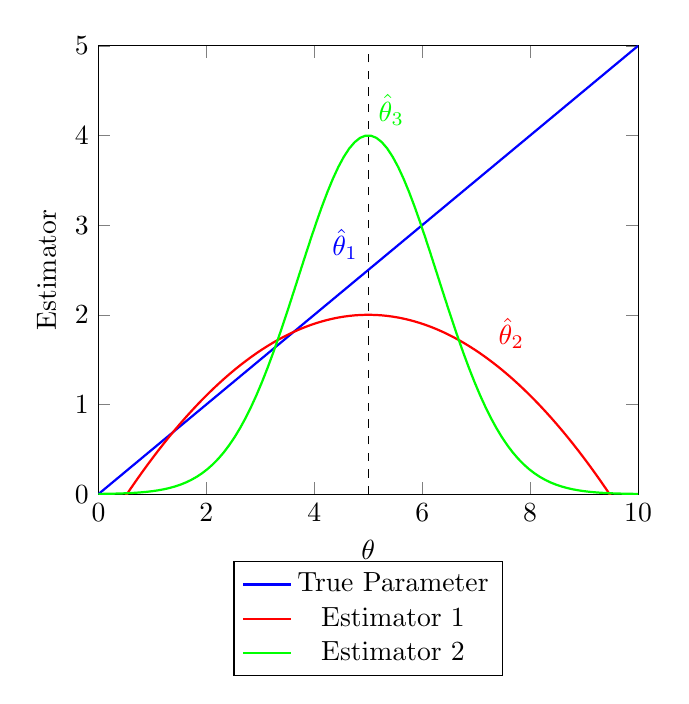
\begin{tikzpicture}
        \begin{axis}[
            xlabel={$\theta$},
            ylabel={Estimator},
            legend style={at={(0.5,-0.15)},anchor=north},
            ymin=0,
            ymax=5,
            xmin=0,
            xmax=10,
            samples=100,
            domain=0:10,
        ]

        % True parameter
        \draw[dashed] (5, 0) -- (5, 5) node[above] {$\theta$};

        % Estimator 1
        \addplot[blue, thick] {0.5*x} node[pos=0.5, above left] {$\hat{\theta}_1$};

        % Estimator 2
        \addplot[red, thick] {2 - 0.1*(x-5)^2} node[pos=0.7, above right] {$\hat{\theta}_2$};

        % Estimator 3
        \addplot[green, thick] {4*exp(-0.3*(x-5)^2)} node[pos=0.5, above right] {$\hat{\theta}_3$};

        \legend{True Parameter, Estimator 1, Estimator 2, Estimator 3}
        \end{axis}
    \end{tikzpicture}
    \caption{Three Possible Estimators}
\end{figure}

\subsubsection{Interval  Estimation: $\sigma^2$ is known }\label{estimationmuknown}
Even the most efficient unbiased estimator is unlikely to precisely estimate the population parameter. Although estimation accuracy improves with larger samples, it is unreasonable to expect a point estimate from a specific sample to exactly match the population parameter it aims to estimate. In many situations, it is preferable to establish an interval within which we anticipate the parameter's value. Such an interval is referred to as an interval estimate.
For example, when estimating a parameter $\Theta$, we assess the probability that this estimation accurately reflects the true value. This probability indicates the extent to which our estimation aligns with the actual parameter. This will be cleared in one example 
\subsubsection{Estimating Mean: $\sigma^2$ is known }

In the previous section, we learned how to calculate the sample mean. The Central Limit Theorem asserts that the distribution of the sample mean approximates a normal distribution with a mean of $\mu$ and a variance of $\sigma^2/n$ means  the spread of the interval for the means is proportional to $\sigma/\sqrt{n}$\\ 
Let's solve an example to get a feel for what it means to estimate the mean with some interval.\\
\begin{example}
    Suppose that if a signal having intensity $\mu$ originates at location A, then the
intensity recorded at location B is normally distributed with mean $\mu$ and
standard deviation 3. That is, due to “noise,” the intensity recorded differs
from the actual intensity of the signal by an amount that is normal with
mean 0 and standard deviation 3. To reduce the error, the same signal is
independently recorded 10 times. If the successive recorded values are
17, 21, 20, 18, 19, 22, 20, 21, 16, 19
construct a 95 percent confidence interval for $\mu$, the actual intensity.
\end{example}
\textbf{Solution}\\
To obtain
such an interval, we start with the sample mean $\Bar{X}$, which is the point estimator
of $\mu$. We now make use of the fact that $\Bar{X}$ is normal with mean $\mu$ and standard 
deviation $\sigma/\sqrt{n}$, which implies that the standardized variable which implies that the standardized variable
$$Z=\frac{\Bar{X}-\mu}{\sigma/\sqrt{n}}=\sqrt{n}\frac{\Bar{X}-\mu}{\sigma}$$ has a standard normal distribution. 
We will use a standard nomenclature for $\alpha = (100 - \text{confidence interval we demand})$. From Figure (7), we see that a 95 percent probability corresponds to $z = 1.96$ (also known as 1.96 standard deviations, equivalent to 2 sigma), which is expressed in statistical nomenclature as $z_{\alpha/2}$.

So, for a 95 percent confidence interval, we can write $z_{\alpha/2} = z_{0.025}$.
Thus we can write
\begin{equation}
    P\{|\frac{\Bar{X}-\mu}{\sigma/\sqrt{n}} |\leq1.96\}=.95
\end{equation}
This gives , 

\begin{equation}
    P\{|\Bar{X}-\mu| \leq 1.96 \frac{\sigma}{n}\}=0.95
\end{equation}
    
From the preceding statement, we see that, with 95 percent probability, $\mu$ and $\Bar{X}$ will be within $1.96\sigma/\sqrt{n}$ of each other. Equivalently,
\begin{equation}
    P\{\Bar{X}-1.96 \frac{\sigma}{\sqrt{n}} \leq \mu \leq \Bar{X}+1.96 \frac{\sigma}{\sqrt{n}}\}=.95
\end{equation}
In general, 
\begin{equation}\label{noramlXFalls}
    P\{\Bar{X}-z_{\alpha/2} \frac{\sigma}{\sqrt{n}} \leq \mu \leq \Bar{X}+z_{\alpha/2}\frac{\sigma}{\sqrt{n}}\}= 1-\alpha
\end{equation}

Now come back to the example 
 Calculate the sample mean $\Bar{X}$
 $$\Bar{X}=\frac{10+17+21+20+18+19+22+20+21+16+19}{10}=19.3$$
 Given $\sigma=3$ following the above discussion , 95 percent confidence interval estimate of $\mu$ is
given by

$$19.3\pm 19.6 \frac{3}{\sqrt{10}}=19.3\pm1.86 $$
SO we can summarise it as follow 

 \fbox{%
\begin{minipage}{\dimexpr\textwidth-2\fboxsep}
\textbf{Confidence interval of $\mu$ Population $\sigma^2$ is Known}\\ 
If $\bar{x}$ is the mean of a random sample of size $n$ from a population with a known variance $\sigma^2$, a $100(1 - \alpha)\%$ confidence interval for $\mu$ is given by
\[
\left(\bar{X} - z_{\alpha/2}\frac{\sigma}{\sqrt{n}} \right) \leq \mu \leq \left(\bar{X} + z_{\alpha/2}\frac{\sigma}{\sqrt{n}} \right),
\]
where $z_{\alpha/2}$ is the z-value leaving an area of $\alpha/2$ to the right.
\end{minipage}%
}
\begin{theorem}
    If $\bar{X}$ is used as an estimate of $\mu$, we can be $100(1 - \alpha)\%$ confident that the error will not exceed $z_{\alpha/2} \sqrt{\frac{\sigma}{n}}$.
\label{thermerro}
\end{theorem}

Sometimes, we wish to know how large a sample is necessary to ensure that the error in estimating $\mu$ will be less than a specified amount $e$. According to Theorem \ref{thermerro}, we must choose $n$ such that $z_{\alpha/2} \frac{\sigma}{\sqrt{ n}} = b$. Solving this equation gives the following formula for $n$.
\begin{theorem}
    If $\bar{X}$ is used as an estimate of $\mu$, we can be $100(1 - \alpha)\%$ confident that the error will not exceed a specified amount $e$ when the sample size is.
    $$n=\left(\frac{z_{\alpha/2}\sigma}{b}\right)^2$$
\end{theorem}
\subsubsection{Mean Estimation: $\sigma$ is unknown}\label{secUnkonwSigma}
In Section (\ref{tdistribution}), we explored the t-distribution. To reiterate, when we have a random sample from a normal distribution, the random variable
\begin{equation}\label{Tform}
    \bar{T} = \frac{\bar{X} - \mu}{S/\sqrt{n}} 
\end{equation}


follows a Student t-distribution with \(n - 1\) degrees of freedom, where \(S\) is the sample standard deviation. In this scenario, when the population standard deviation \(\sigma\) is unknown, \(\bar{T}\) can be utilized to construct a confidence interval for \(\mu\). The procedure is analogous to that when \(\sigma\) is known, except that \(\sigma\) is replaced by \(S\), and the standard normal distribution is replaced by the t-distribution. So whatever we did in section(\ref{estimationmuknown}) we will do the same but,  with t-dstribution. In the case of t-dsitribtuin formula (\ref{noramlXFalls}) will take the following form 
\begin{equation}\label{TdistlXFalls}
    P\{\Bar{X}-t_{n-1,\alpha/2} \frac{S}{\sqrt{n}} \leq \mu \leq \Bar{X}+t_{n-1,\alpha/2}\frac{S}{\sqrt{n}}\}= 1-\alpha
\end{equation}


 \fbox{%
\begin{minipage}{\dimexpr\textwidth-2\fboxsep}
\textbf{Confidence interval of $\mu$ Population $\sigma^2$ is unknown}\\ 
If $\bar{x}$ and $s$ are the mean and standard deviation of a random sample from a normal population with an unknown variance $\sigma^2$, a $100(1 - \alpha)\%$ confidence interval for $\mu$ is

\[ \bar{x} - t_{\alpha/2}\frac{s}{\sqrt{n}} < \mu < \bar{x} + t_{\alpha/2}\frac{s}{\sqrt{n}}, \]

where $t_{\alpha/2}$ is the t-value with \(v = n - 1\) degrees of freedom, leaving an area of $\alpha/2$ to the right.

\end{minipage}%
}

\fbox{%
\begin{minipage}{\dimexpr\textwidth-2\fboxsep}
\textbf{Concept}

    Often, statisticians recommend that even when normality cannot be assumed, \(\sigma\) is unknown, and \(n \geq 30\), \(s\) can replace \(\sigma\), and the confidence interval

\[ \bar{x} \pm z_{\alpha/2} \frac{s}{\sqrt{n}} \]

may be used. This is often referred to as a large-sample confidence interval. The justification lies only in the presumption that with a sample as large as 30 and the population distribution not too skewed, \(s\) will be very close to the true \(\sigma\), and thus the Central Limit Theorem prevails. It should be emphasized that this is only an approximation, and the quality of the result becomes better as the sample size grows larger.

\end{minipage}
}
\subsubsection{Interval of Estimators of a Large Population}
So far, we have estimated the population parameter $\mu$ or $\sigma$. Now, we will consider how to estimate the probability that an individual in the population possesses a certain characteristic..
Imagine you're interested in figuring out the proportion of individuals in a large population who possess a certain characteristic, such as owning a specific brand of smartphone. To estimate this proportion, you take a random sample of individuals from the population, and let's say there are $n$ people in your sample.\\

Now, you observe how many individuals in your sample actually have the characteristics you're interested in. Let's call this number $X$. The sample proportion ($\hat{p}$) is then calculated by dividing the number of individuals with the characteristic $X$ by the total sample size $n$. Mathematically, it's represented as $\hat{p}=\frac{X}{n}$.\\

This sample proportion $\hat{p}$ serves as an estimate of the true proportion $p$ in the entire population. Essentially, you're using information from your sample to make an educated guess about the proportion of the entire population that possesses the characteristic.\\

If we let $X$ denote the number of members of the population who have the
characteristic, then it follows from the preceding that if the population size N
is large in relation to the sample size $n$, then the distribution of X is approxi-
mately a binomial distribution with parameters $n$ and $p$.\\\
We know the mean and standard deviation of a binomial random variable
\[
E[X] = np \quad \text{and} \quad SD(X) = \sqrt{np(1 - p)}
\]
Since $\Bar{X}$, the proportion of the sample that has the characteristic is equal to \(\frac{X}{n}\), we see that
\[
E\left[\frac{\Bar{X}}{n}\right] = p \quad \text{and} \quad SD(\bar{X})=\frac{SD(X)}{n} = \frac{\sqrt{p(1 - p)}}{n}
\]
When \(n\) is large enough that both \(np\) and \(n(1 - p)\) are greater than 5, we can use the normal approximation to the binomial distribution to assert that an approximate \(100(1 - \alpha)\) percent confidence interval estimator of \(p\) is given by
\[ \hat{p} \pm z_{\alpha/2} \cdot \text{SD}(\hat{p}) \]

Although the standard deviation of \(\hat{p}\) is not known since it involves the unknown proportion \(p\), we can estimate it by replacing \(p\) by its estimator \(\hat{p}\) in the expression for \(\text{SD}(\hat{p})\). That is, we can estimate \(\text{SD}(\hat{p})\) by \(\sqrt{\hat{p}(1 - \hat{p})/n}\). This gives rise to the following.

\fbox{
  \begin{minipage}{\dimexpr\textwidth-2\fboxsep}\textbf{Interval estimator of population proportion}
    An approximate \(100(1 - \alpha)\) percent confidence interval estimator of \(p\) is given by
    \[
      \hat{p} - z_{\alpha/2} \sqrt{\frac{\hat{p}(1 - \hat{p})}{n}}\leq p \leq\hat{p} + z_{\alpha/2} \sqrt{\frac{\hat{p}(1 - \hat{p})}{n}}
    \]
    where \(\hat{p}\) is the proportion of members of the sample of size \(n\) who have the characteristic of interest.
  \end{minipage}
}
\begin{example}\citep{ross2017introductory}
    Out of a random sample of 100 students at a university, 82 stated that they were nonsmokers. Based on this, construct a 99 percent confidence interval estimate of \(p\), the proportion of all the students at the university who are nonsmokers.

\textbf{Solution:}
Since \(100(1 - \alpha) = 0.99\) when \(\alpha = 0.01\), we need the value of \(z_{\alpha/2} = z_{0.005}\), which from Table D.2 is equal to 2.576. The 99 percent confidence interval estimate of \(p\) is thus
\[
0.82 \pm 2.576 \sqrt{\frac{0.82(1 - 0.82)}{100}}
\]
or
\[
0.82 \pm 0.099
\]
That is, we can assert with 99 percent confidence that the true percentage of nonsmokers is between 72.1 and 91.9 percent.

\end{example}

 \begin{example}
     \citep{ross2017introductory}
     On December 24, 1991, The New York Times reported that a poll indicated that 46 percent of the population was in favor of the way that President Bush was handling the economy, with a margin of error of ±3 percent. What does this mean? Can we infer how many people were questioned?

\textbf{Solution:}
It has become common practice for the news media to present 95 percent confidence intervals. That is, unless it is specifically mentioned otherwise, it is almost always the case that the interval quoted represents a 95 percent confidence interval. Since \(Z_{0.025} = 1.96\), a 95 percent confidence interval for \(p\) is given by
\[
\hat{p} \pm 1.96 \sqrt{\frac{\hat{p}(1 - \hat{p})}{n}}
\]
where \(n\) is the sample size. Since \(\hat{p}\), the proportion of those in the random sample who are in favor of the President’s handling of the economy, is equal to 0.46, it follows that the 95 percent confidence interval estimate of \(p\), the proportion of the population in favor, is
\[
(0.46) \pm 1.96 \sqrt{\frac{(0.46)(0.54)}{n}}
\]

Since the margin of error is ±3 percent, it follows that
\[
(0.46)(0.54) = 0.03 \times 1.96 \times n
\]

Squaring both sides of this equation shows that
\[
n = \frac{(1.96)^2 (0.46)(0.54)}{(0.03)^2} = 1060.3
\]

That is, approximately 1060 people were sampled, and 46 percent were in favor of President Bush’s handling of the economy.

 \end{example}
\subsubsection{Estimation of mean for two populations}
If we have two populations with means \(\mu_1\) and \(\mu_2\) and variances \(\sigma_1^2\) and \(\sigma_2^2\), respectively, a point estimator of the difference between \(\mu_1\) and \(\mu_2\) is given by the statistic \(\bar{X}_1 - \bar{X}_2\). Therefore, to obtain a point estimate of \(\mu_1 - \mu_2\), we shall select two independent random samples, one from each population, of sizes \(n_1\) and \(n_2\), and compute \(\bar{x}_1 - \bar{x}_2\), the difference of the sample means. So the estimation formula will follow exactly the equation (\ref{noramlXFalls})
\fbox{
  \begin{minipage}{\dimexpr\textwidth-2\fboxsep}\textbf{confidence interval for the difference of mean when SD of both population is known}\\
    \citep{walpole1993probability}If \(\bar{x}_1\) and \(\bar{x}_2\) are means of independent random samples of sizes \(n_1\) and \(n_2\) from populations with known variances \(\sigma_1^2\) and \(\sigma_2^2\), respectively, a \(100(1 - \alpha)\%\) confidence interval for \(\mu_1 - \mu_2\) is given by
    \[
     (\bar{x}_1 - \bar{x}_2) - z_{\alpha/2} \sqrt{\frac{\sigma_1^2}{n_1^2} + \frac{\sigma_2^2}{n_2^2}} < \mu_1 - \mu_2 <  (\bar{x}_1 - \bar{x}_2) + z_{\alpha/2} \sqrt{\frac{\sigma_1^2}{n_1^2} + \frac{\sigma_2^2}{n_2^2}} 
    \]
    where \(z_{\alpha/2}\) is the z-value leaving an area of \(\alpha/2\) to the right.
  \end{minipage}
}

\subsubsection{Interval Estimation of two populations unknown SD's  }
 In the case where the variances of populations are not known, as discussed in Section~\ref{secUnkonwSigma}, we learned how to estimate intervals using the Student's t-distribution. When dealing with two different populations, the argument and formula remain the same form as in the aforementioned section, with the only difference being the presence of two means (\(\mu\)'s).
 The variance of samples pooled from two populations will be (for further derivation \citep{walpole1993probability}
\begin{equation}
    S_p^2=\frac{(n_1-1)S_1^2+(n_2-1)S_2^2}{n_1+n_2-2}
\end{equation}
 $S_p$ p subscript stands for pooled variance 
The student t- distribution in this case will take as following form,
\begin{equation}
    T=\frac{\Bar{X}_{1}-\Bar{X}_{1}}{S_p \sqrt{1/n_1+1/n_2}}
\end{equation}
Using the T statistic, we have
\begin{equation}
    P\left(-t_{\alpha/2} < T < t_{\alpha/2}\right) = 1 - \alpha,
\end{equation}


where \(t_{\alpha/2}\) is the t-value with \(n_1 + n_2 - 2\) degrees of freedom, above which we find an area of \(\alpha/2\). So, interval estimator from equation (\ref{TdistlXFalls}) will be 
\begin{equation}
    P\{(\Bar{X_1}-\Bar{X_2})-t_{\alpha/2}\frac{S_p}{\sqrt{1/n_1+1/n_2}}\leq(\mu_1-\mu_2)\leq(\Bar{X_1}-\Bar{X_2})-t_{\alpha/2}\frac{S_p}{\sqrt{1/n_1+1/n_2}}\}=1-\alpha
\end{equation}

\fbox{
 \begin{minipage}{\dimexpr\textwidth-2\fboxsep}
 \textbf{Confidence interval for $\mu_1-\mu_1$ : variances are unknown and equal}
    If \(\bar{x}_1\) and \(\bar{x}_2\) are the means of independent random samples of sizes \(n_1\) and \(n_2\), respectively, from approximately normal populations with unknown but equal variances, a \(100(1 - \alpha)\%\) confidence interval for \(\mu_1 - \mu_2\) is given by
   
    \[
      (\bar{x}_1 - \bar{x}_2) - t_{\alpha/2} s_p \sqrt{\frac{1}{n_1} + \frac{1}{n_2}} < \mu_1 - \mu_2 < (\bar{x}_1 - \bar{x}_2) + t_{\alpha/2} s_p \sqrt{\frac{1}{n_1} + \frac{1}{n_2}},
    \]
    where \(s_p\) is the pooled estimate of the population standard deviation and \(t_{\alpha/2}\) is the t-value with \(v = n_1 + n_2 - 2\) degrees of freedom, leaving an area of \(\alpha/2\) to the right.
  \end{minipage}
}
\subsection{Interval Estimation of variance }
We are familiar with how to estimate the variance of a population using the formula \ref{meandef}. Now, our objective is to calculate the confidence interval for the estimated variance. To summarize our approach: first, we estimated the mean, and subsequently, to determine the confidence interval for the mean, we required the distribution of the mean. This distribution function played a crucial role in defining the length of the confidence interval. Similarly, we will follow a comparable process to estimate the confidence interval for the variance. Therefore, we need to identify a distribution that can closely approximate the distribution of the variance  $S^2$, sample variance. 
We say we want the distribution function of
$$X^2\sim S^2$$
The theorem (\ref{chitheorem}) allows us to have such distribution 
An interval estimate of $\sigma^2$ can be established by using the statistic $X^2 = \frac{(n - 1)S^2}{\sigma^2}$. \citep{walpole1993probability}
\begin{center}
\fbox{
    \begin{minipage}{\dimexpr\textwidth-2\fboxsep}
        If $s^2$ is the variance of a random sample of size $n$ from a normal population, a $100(1 - \alpha)\%$ confidence interval for $\sigma^2$ is
        \[
            \frac{(n - 1)s^2}{\chi^2_{\alpha/2}} < \sigma^2 < \frac{(n - 1)s^2}{\chi^2_{1 - \alpha/2}},
        \]
        where $\chi^2_{\alpha/2}$ and $\chi^2_{1-\alpha/2}$ are $\chi^2$-values with $v = n - 1$ degrees of freedom, leaving areas of $\alpha/2$ and $1 - \alpha/2$ to the right.
    \end{minipage}
}
\end{center}
\subsubsection{Maximum Likelihood Method}
\section{Hypothesis testing: One-population and Two- population}
Hypothesis testing is a type of statistical inference that is used to determine whether there is enough evidence to support a particular claim about a population parameter. For example, you might hypothesize that the average size of all the marbles in the bag is 1 inch. You would then collect data on the size of a sample of marbles and use a statistical test to determine whether there is enough evidence to reject the hypothesis that the average size is 1 inch.

There are two types of errors that can occur in hypothesis testing:

    Type I error: This is when you reject the null hypothesis (the hypothesis that the population parameter is a certain value) even though it is actually true.
    Type II error: This is when you fail to reject the null hypothesis even though it is actually false.

The goal of hypothesis testing is to minimize the risk of both type I and type II errors. This is done by setting a significance level, which is the maximum probability of making a type I error that you are willing to accept. The significance level is typically set at 0.05 or 0.01.
\begin{definition}
    The null hypothesis, denoted by $H_0$, is a statement about a population parameter. The alternative
hypothesis is denoted by $H_1$ The null hypothesis will be rejected if it appears to be inconsistent
with the sample data and will not be rejected otherwise.
\end{definition}
\section{Analysis-of-Variance Technique}
progress
\section{ Linear Regression and Correlation}
Progress...
\section{Bayesian Inference}
Progress


\section{A brief Sketch of Application in Experimental Particle Phyiscs}
Progress
\bibliographystyle{apalike}
\bibliography{example}

\end{document}